%%%%%%%%%%%%%%%%%%%%%%%%%%%%%%%%%%%%%%%%%
% Masters/Doctoral Thesis 
% LaTeX Template
% Version 2.4 (22/11/16)
%
% This template has been downloaded from:
% http://www.LaTeXTemplates.com
%
% Version 2.x major modifications by:
% Vel (vel@latextemplates.com)
%
% This template is based on a template by:
% Steve Gunn (http://users.ecs.soton.ac.uk/srg/softwaretools/document/templates/)
% Sunil Patel (http://www.sunilpatel.co.uk/thesis-template/)
%
% Template license:
% CC BY-NC-SA 3.0 (http://creativecommons.org/licenses/by-nc-sa/3.0/)
%
%%%%%%%%%%%%%%%%%%%%%%%%%%%%%%%%%%%%%%%%%

%----------------------------------------------------------------------------------------
%	PACKAGES AND OTHER DOCUMENT CONFIGURATIONS
%----------------------------------------------------------------------------------------

\documentclass[
11pt, % The default document font size, options: 10pt, 11pt, 12pt
oneside, % Two side (alternating margins) for binding by default, uncomment to switch to one side
ngerman, 
singlespacing, % Single line spacing, alternatives: onehalfspacing or doublespacing
%draft, % Uncomment to enable draft mode (no pictures, no links, overfull hboxes indicated)
%nolistspacing, % If the document is onehalfspacing or doublespacing, uncomment this to set spacing in lists to single
%liststotoc, % Uncomment to add the list of figures/tables/etc to the table of contents
%toctotoc, % Uncomment to add the main table of contents to the table of contents
parskip, % Uncomment to add space between paragraphs
%nohyperref, % Uncomment to not load the hyperref package
headsepline, % Uncomment to get a line under the header
chapterinoneline, % Uncomment to place the chapter title next to the number on one line
%consistentlayout, % Uncomment to change the layout of the declaration, abstract and acknowledgements pages to match the default layout
]{MastersDoctoralThesis} % The class file specifying the document structure

\usepackage[utf8]{inputenc} % Required for inputting international characters
\usepackage[T1]{fontenc} % Output font encoding for international characters

\usepackage{palatino} % Use the Palatino font by default

\usepackage[backend=bibtex,style=numeric,natbib=true]{biblatex} % Use the bibtex backend with the authoryear citation style (which resembles APA)

\addbibresource{bibliography.bib} % The filename of the bibliography

\usepackage[autostyle=true]{csquotes} % Required to generate language-dependent quotes in the bibliography

\usepackage{microtype}
\usepackage{pdfpages}
\usepackage{graphicx}
\usepackage[font=it]{caption}

\usepackage{listings}
\lstdefinelanguage{VHDL}{
   morekeywords={
     library,use,all,entity,is,port,in,out,end,architecture,of,
     begin,and
   },
   morecomment=[l]--
}

\lstdefinestyle{vhdl}{
   language     = VHDL,
   basicstyle   = \ttfamily,
   keywordstyle = \color{keyword}\bfseries,
   commentstyle = \color{comment}
}

% command \code{Text}
%\newcommand{\code}[1]{\texttt{#1}}

%----------------------------------------------------------------------------------------
%	MARGIN SETTINGS
%----------------------------------------------------------------------------------------

\geometry{
	paper=a4paper, % Change to letterpaper for US letter
	inner=2.5cm, % Inner margin
	outer=3.8cm, % Outer margin
	bindingoffset=.5cm, % Binding offset
	top=1.5cm, % Top margin
	bottom=1.5cm, % Bottom margin
	%showframe, % Uncomment to show how the type block is set on the page
}

%----------------------------------------------------------------------------------------
%	THESIS INFORMATION
%----------------------------------------------------------------------------------------

\thesistitle{Implementierung der RISC-V Spezifikation auf einem FPGA in VHDL} % Your thesis title, this is used in the title and abstract, print it elsewhere with \ttitle
\supervisor{Prof. Dr. \textsc{Reith}} % Your supervisor's name, this is used in the title page, print it elsewhere with \supname
\examiner{} % Your examiner's name, this is not currently used anywhere in the template, print it elsewhere with \examname
\degree{} % Your degree name, this is used in the title page and abstract, print it elsewhere with \degreename
\author{Andreas \textsc{Rollbühler},\\ Jens \textsc{Nazarenus},\\ Nils \textsc{Geiselhart}} % Your name, this is used in the title page and abstract, print it elsewhere with \authorname
\addresses{} % Your address, this is not currently used anywhere in the template, print it elsewhere with \addressname

\subject{Informatik} % Your subject area, this is not currently used anywhere in the template, print it elsewhere with \subjectname
\keywords{} % Keywords for your thesis, this is not currently used anywhere in the template, print it elsewhere with \keywordnames
\university{\href{https://www.hs-rm.de/de/}{Hochschule RheinMain}} % Your university's name and URL, this is used in the title page and abstract, print it elsewhere with \univname
\department{\href{https://www.hs-rm.de/de/fachbereiche/design-informatik-medien/aktuelles/}{Fachbereich Design Informatik Medien}} % Your department's name and URL, this is used in the title page and abstract, print it elsewhere with \deptname
\group{\href{}{}} % Your research group's name and URL, this is used in the title page, print it elsewhere with \groupname
\faculty{\href{}{}} % Your faculty's name and URL, this is used in the title page and abstract, print it elsewhere with \facname

\AtBeginDocument{
\hypersetup{pdftitle=\ttitle} % Set the PDF's title to your title
\hypersetup{pdfauthor=\authorname} % Set the PDF's author to your name
\hypersetup{pdfkeywords=\keywordnames} % Set the PDF's keywords to your keywords
}

\begin{document}

\frontmatter % Use roman page numbering style (i, ii, iii, iv...) for the pre-content pages

\pagestyle{plain} % Default to the plain heading style until the thesis style is called for the body content

%----------------------------------------------------------------------------------------
%	TITLE PAGE
%----------------------------------------------------------------------------------------

\begin{titlepage}
\begin{center}

\vspace*{.06\textheight}
{\scshape\LARGE \univname\par}\vspace{1.5cm} % University name
\textsc{\Large Projektdokumentation}\\[0.5cm] % Thesis type

\HRule \\[0.4cm] % Horizontal line
{\huge \bfseries \ttitle\par}\vspace{0.4cm} % Thesis title
\HRule \\[1.5cm] % Horizontal line
 
\begin{minipage}[t]{0.4\textwidth}

\begin{flushleft} \large
\emph{Autoren:}\\
\authorname % Author name - remove the \href bracket to remove the link
\end{flushleft}
\end{minipage}
\begin{minipage}[t]{0.4\textwidth}
\begin{flushright} \large
\emph{Projektbetreuer:} \\
\href{https://www.cs.hs-rm.de/~reith/}{\supname} % Supervisor name - remove the \href bracket to remove the link  
\end{flushright}
\end{minipage}\\[3cm]
 
\vfill

\large \textit{Dokumentation der Praktischen Tätigkeit\\ im Rahmen des Wahlprojekts Hardware/Software-Schnittstellen\\ im Wintersemester 2016/1017}
\\[1cm] % University requirement text
%\textit{im}\\[0.4cm]
%\groupname\\\deptname\\[2cm] % Research group name and department name
 
\vfill

{\large \today}\\[2cm] % Date

\includegraphics[scale=0.8]{HSRM_logo} % University/department logo - uncomment to place it
 
\vfill
\end{center}
\end{titlepage}

%----------------------------------------------------------------------------------------
%	ABSTRACT PAGE
%----------------------------------------------------------------------------------------

\begin{abstract}
\addchaptertocentry{\abstractname} % Add the abstract to the table of contents

Dieses Dokument wurde im Rahmen des Wahlprojekts \textit{Software- Hardwareschnittstellen} bei Prof. Dr. \emph{Reith} an der Hochschule RheinMain verfasst. 

Es dokumentiert die Konzeptionalisierung und die Implementierung einer CPU auf einem \textit{FPGA} Board. Die verwendete Befehlssatzarchitektur basiert auf dem offenen \textit{\href{https://riscv.org/}{RISC-V}} Design. Die Architektur wurde unter Verwendung der Hardwarebeschreibungssprache \textit{VHDL} implementiert. Anschließend wurde sie testweise für das \textit{\href{https://reference.digilentinc.com/reference/programmable-logic/nexys-4/start}{Xilinx Nexys 4\textsuperscript{\textregistered}}} Board mit Artix-7\textsuperscript{\textregistered} \emph{FPGA} synthetisiert.

Ferner dokumentiert diese Arbeit das Projekt- und Teammanagement. Sie beschreibt die Verwendung von Versionskontrollsystemen, den Workflow und die Testumgebung im Zusammenhang mit der VHDL-Entwicklungsumgebung \textit{Xilinx} \textit{\href{https://www.xilinx.com/products/design-tools/vivado.html}{Vivado\textsuperscript{\textregistered} Design Suite}}.

Das umgesetzte Projekt ist unter der GPL3-Lizenz veröffentlicht das Repository \ref{???} frei verfügbar.
 
\end{abstract}

%----------------------------------------------------------------------------------------
%	LIST OF CONTENTS
%----------------------------------------------------------------------------------------

\let\cleardoublepage\clearpage 
\tableofcontents % Prints the main table of contents

%\listoffigures % Prints the list of figures

%\listoftables % Prints the list of tables

%----------------------------------------------------------------------------------------
%	THESIS CONTENT - CHAPTERS
%----------------------------------------------------------------------------------------

\mainmatter % Begin numeric (1,2,3...) page numbering

\pagestyle{thesis} % Return the page headers back to the "thesis" style

% Include the chapters of the thesis as separate files from the Chapters folder
% Uncomment the lines as you write the chapters

\chapter{Einleitung} % Main chapter title
\label{Einleitung} % For referencing the chapter elsewhere, use \ref{Chapter1} 

%----------------------------------------------------------------------------------------

% Define some commands to keep the formatting separated from the content 
\newcommand{\keyword}[1]{\textbf{#1}}
\newcommand{\tabhead}[1]{\textbf{#1}}
\newcommand{\code}[1]{\texttt{#1}}
\newcommand{\file}[1]{\texttt{\bfseries#1}}
\newcommand{\option}[1]{\itshape#1}

Diese Arbeit wurde im Rahmen des Wahlprojekts \textit{Software- Hardwareschnittstellen} bei Prof. Dr. \emph{Reith} an der Hochschule RheinMain verfasst. Die vorgegebene Projektaufgabe beinhaltet die Implementierung einer CPU auf einem \emph{FPGA} mittels der Hardwarebeschreibungssprache \emph{VHDL}. Die CPU soll die offene \emph{RISV-V} Architektur umsetzen. Diese Dokumentation beschreibt das Konzept, die Planung und die Umsetzung dieser Aufgabenstellung.

Zunächst werden hierfür einige allgemeine Grundbegriffe, die zum Verständnis des Projekts erforderlich sind, kurz erläutert: Die FPGA-Technologie, die Hardwarebeschreibungssprache VHDL, die offene Befehlssatzarchitektur RISC-V und welche Teilmenge des (modularen) RISC-V Befehlssatzes umgesetzt wurde. Dabei soll jedoch lediglich ein kurzer Überblick über die Materie verschafft werden. Für das tiefere Verständnis und Anleitungen sei auf die entsprechende Fachliteratur für VHDL\citep{Ashenden:609207}, FPGA-Programmierung\cite{Chu} mit Vivado\cite{churiwala} und auf die RISC-V Spezifikation\citep{RISC} verwiesen.

Der Schwerpunkt liegt stattdessen auf der Beschreibung der Umsetzung der gesetzten Aufgabenstellung. Dafür wurde in Kapitel \ref{Umsetzung} die konkrete Implementierung der einzelnen Komponenten der RISC-V CPU in VHDL dokumentiert. Anschließend stellt Kapitel \ref{organisation} die Herausforderungen des Team- und Projektmanangements dar und wie mit ihnen umgegangen wurde. Es wird die Arbeitsteilung, die Versionskontrolle mit \emph{git} und die Qualitätssicherung durch Softwaretests beschrieben.

Kapitel \ref{Probleme} dokumentiert die Herausforderungen, auf die das Team im Laufe der Entwicklung gestoßen ist und inwiefern dadurch Teile der Umsetzung limitiert oder eingeschränkt werden mussten. Es werden außerdem mögliche Lösungsansätze diskutiert. Ferner wird ein kurzer Ausblick auf künftige Entwicklungen des Projekts gegeben.

Schließlich werden in Kapitel \ref{Ergebnis} die Ergebnisse der Arbeit zusammengefasst dargestellt und die Details und Kennwerte der umgesetzten CPU aufbereitet. 

Das Ergebnis dieser Arbeit ist unter \ref{???} frei verfügbar.
 %Einleitung
\chapter{FPGA} % Main chapter title
\label{FPGA} % For referencing the chapter elsewhere, use \ref{Chapter1} 

Ein FPGA (Field Programmable Gate Array) ist ein Schaltkreis, in den eine beliebige logische Schaltung programmiert werden kann. Der Vorteil besteht dabei insbesondere darin, dass FPGA's beliebig oft neu programmiert werden können. 

%----------------------------------------------------------------------------------------
\section{Technik}

%---------------------------------------------------------------------------------------- %FPGA
\chapter{VHDL} % Main chapter title
\label{VHDL} % For referencing the chapter elsewhere, use \ref{Chapter1} 

%----------------------------------------------------------------------------------------
\section{Einleitung}
VHDL (\textit{Very High Speed Integrated Circuit Hardware Description Language}) ist eine Hardwarebeschreibungssprache, die 1980 entwickelt wurde. Mit ihr kann das Verhalten einer logischen Schaltung formalisiert textuell beschrieben werden. 

Anstatt eine Schaltung aus ihren einzelnen elektronischen Teilen zu entwerfen, arbeitet VHDL auf einer höheren Abstraktionsschicht. Es wird lediglich beschrieben, wie sich eine Schaltung oder ein logischer Teil einer Schaltung in Abhängigkeit bestimmter Eingangsgrößen verhält.
%----------------------------------------------------------------------------------------

%----------------------------------------------------------------------------------------
\section{Entwicklung mit VHDL}
\paragraph{Entities.} In VHDL werden \textit{Entities} definiert, die eine Klasse von Schaltelementen repräsentieren. Entities bestehen üblicherweise aus mehreren Ein-und Ausgangs\textit{ports}. Innerhalb der \textit{Architecture} einer \textit{Entity} wird festgelegt, wie sich die Ausgangssignale in Abhängigkeit der Eingangssignale verhalten.

\paragraph{Parallelität.} Bei der Entwicklung ist insbesondere zu beachten, dass das Verhalten einer Entity, anders als von Programmiersprachen gewohnt, im Allgemeinen nicht sequentiell abgearbeitet wird. Vielmehr findet die Signalverarbeitung parallel statt.

\paragraph{Processes.} Innerhalb des Verhaltens können deshalb Prozesse deklariert werden, deren Instruktionen sequentiell abgearbeitet werden. Zu diesem Zweck können innerhalb eines Prozesses auch \textit{Variablen} verwendet werden.

\paragraph{Strukturmodelle.} Neben Verhaltensmodellen kann mit Strukturmodellen eine Schaltung aus mehreren Entities beschrieben werden. Dafür werden sog. \textit{Components} (Instanzen von zuvor beschriebenen Entities) erstellt und deren Ports miteinander verbunden.

So können verhältnismäßig einfach komplexe Verschaltungen beschrieben werden.
%----------------------------------------------------------------------------------------
 
%----------------------------------------------------------------------------------------
\section{Umsetzung von VHDL}
Auf die konkrete Umsetzung der beschriebenen Schaltung hat der Anwender dabei nur bedingten Einfluss, da die Implementierung der Schaltung in Hardware selbst üblicherweise von automatisierten Werkzeugen durchgeführt wird. Dabei lassen sich mehrere Schritte unterscheiden. In diesem Projekt wurde die Entwicklungsumgebung Vivado Design Suite von Xilinx verwendet, um den VHDL-Code umzusetzen.

\paragraph{Simulation.} In einem ersten Schritt kann der VHDL Code \emph{simuliert} werden, was vor allem in der Testphase von Bedeutung ist. Dabei wird der Code noch nicht auf der Hardware ausgeführt, sondern das Verhalten der Schaltung mittels sogenannter Testbenches simuliert, die die Schaltung mit virtuellen Eingangssignalen (z. B. Taktrate) versorgen. 

TODO: Screenshot?

\paragraph{Synthese.} Das simulierte Verhalten kann anschließend \emph{synthetisiert} werden. Dabei ist zu beachten, dass nicht die vollständige Menge von zulässigem (und simulationsfähigem) VHDL-Code letztlich in eine physische Schaltung synthetisierbar ist (so z. B. \emph{wait}-Statements). Das ist abhängig von der verwendeten Zieltechnologie (FPGA, ASIC) und dem verwendeten Synthesetool. Das Ergebnis der Synthese ist eine Netzliste, die einer textuellen Beschreibung des umgesetzten Schaltplans entspricht.

\paragraph{Implementierung.} Diese Netzliste ist Grundlage der Hardwareimplementierung. Dabei wird innerhalb des \emph{place and route} Vorgangs unter Berücksichtigung der verfügbaren Hardware und bestimmter zeitlicher Beschränkungen berechnet, wo die einzelnen Schaltelemente auf der Hardware implementiert werden und wie sie verbunden werden.
%----------------------------------------------------------------------------------------
 %VHDL
\chapter{RISC-V} % Main chapter title
\label{RISC-V} % For referencing the chapter elsewhere, use \ref{Chapter1} 

\section{Einleitung}
\emph{RISC-V} ist eine offene Befehlssatzarchitektur, die 2010 von Entwicklern an der University of California, Berkeley vorgestellt wurde. Sie basiert auf der RISC (reduced instruction set computing) Design\textit{philosophie} basiert. 

???Falsch: In Abgrenzung zu CISC (complex instruction set computing) sind RISC Befehlssätze leichtgewichtiger, d. h. es werden in der Regel weniger Maschineninstruktionen definiert. ??Vor-Nachteile?

Ein wichtiger Vorteil von RISC-Architekturen, insbesondere im Hinblick auf das vorliegende Projekt, liegt in der einfachen Implementierung. 

Beim Entwurf wurde besonderer Wert auf eine leichtgewichtige Architektur, aber auch Performance und Energiesparsamkeit gelegt.

Eine Befehlssatzarchitektur definiert den Befehlssatz einer CPU. Sie spezifiziert u. a., welche Maschinenbefehle eine CPU verarbeiten können muss, was genau ihre Ausführung bewirkt wie sie mit dem Speicher interagiert und definiert und wie definiert CPU eigene Speicherbänke (Register). Sie stellt damit die Schnittstelle zwischen der Hardware und Software einer Maschine dar. Mithilfe einer solchen einheitlichen Schnittstelle kann Software ohne Kenntnis der zugrunde liegenden Hardware Software für eine Maschine programmieren.

Von der Befehlssatzarchitektur abzugrenzen ist die Mikroarchitektur, die die Implementierung des Befehlssatzes auf einem Chip bestimmt.

Für dieses Projekt wurde der RISC-V (Link?!) Befehlssatz übernommen, und eine eigene Hardware-Implementierung, die die Befehlssatzspezifikation von RISC-V erfüllt, entwickelt.


%----------------------------------------------------------------------------------------
\section{RISC-V Varianten und verwendetes Instruktionssubset}

\paragraph{Wortbreite.} Für RISC-V Architekturen sind die Wortbreiten $32, 64$ und $128$bit vorgesehen.

\paragraph{Erweiterungen.} Die RISC-V Architektur ist darauf ausgelegt, flexibel erweiterbar zu sein. Die Spezifikation definiert daher mehrere Teilmengen des allgemeinen Befehlssatzes. \citep[p. 4]{RISC}

Um die RISC-V Anforderungen zu erfüllen, muss eine Implementierung zumindest die Basisinstruktionen zur Integerverarbeitung umsetzen (Bezeichnung nach RISC-V Konvention: \textit{I})

Die allgemeine als \textit{General Purpose} bezeichnete Architektur enthält neben diesem Mindeststandard auch Befehle für Gleitkommaarithmetik (F) mit Double(D) oder Quad-Präzision (Q), für die Handhabung verschiedener Privilegierungen (P), atomare Befehle für die Verwaltung von Nebenläufigkeit (A) und seit der neusten Version 2.1 auch für Bitmanipulation (B), Vectoroperationen (V) und einigen mehr.

\paragraph{Verwendetes Subset.} In diesem Projekt wurde sich allerdings darauf beschränkt, eine einfache integerverarbeitende Mikroarchitektur umzusetzen. Als Wortbreite wurden 32bit gewählt. Die Bezeichnung des verwendeten Subsets lautet daher nach RISC-V Konventionen \textit{RV32I}.
%----------------------------------------------------------------------------------------

%----------------------------------------------------------------------------------------
\section{RV32I}
Das verwendete Subset besteht aus $47$ verschiedenen Maschineninstruktionen.

\begin{figure} [ht]
  \centering
  \includegraphics[width=0.95\textwidth]{Figures/instruction_formats}
  \caption{Instruktionsformate. Quelle: \citep[p. 11]{RISC}}
  \label{fig:instr_types}
\end{figure}

\subsection{Register}
???

\subsection{Instruktionsformate}
RV32I kennt vier verschiedene Formate, in denen Maschinen instruktionen enkodiert sein können: \textit{R-type}, \textit{I-Type}, \textit{S-type} und \textit{U-type} - Befehle.

%----------------------------------------------------------------------------------------

%----------------------------------------------------------------------------------------
\section{Architektur}
- branch delay slots?
\subsection{Speicherarchitektur}
RISC-V ist als \textit{load-store}-Architektur entworfen. Arithmetische und logische Instruktionen greifen daher nicht auf den Speicher zu, stattdessen werden alle Operatoren vorher in der Registerbank abgelegt. Rechenergebnisse werden ebenfalls in Registern gespeichert. Speicherzugriffe werden ausschließlich mit \textit{load} bzw. \textit{store}-Befehlen realisiert.

\subsection{Register}
Die RISC-V Spezifikation definiert 31 Integer Register 1 - 31. Zusätzlich existiert ein \textit{zero}-Register, das eine konstante 0 beinhaltet. Andere Register (Floating Point) können an dieser Stelle vernachlässigt werden, da sich die umgesetzte CPU auf Integerverarbeitung beschränkt.
%----------------------------------------------------------------------------------------

%----------------------------------------------------------------------------------------
\section{Maschinenbefehle}
RISC-V Maschinenbefehle haben eine fixe Länge, die der Wortlänge der Architektur entspricht?
\paragraph{Branches.} Branches blabla ed diam nonumy eirmod tempor invidunt ut labore et dolore magna aliquyam erat, sed diam voluptua. At vero eos et accusam et justo duo dolores et ea rebum. Stet clita kasd gubergren, no sea takimata sanctus est Lorem ipsum dolor sit amet.
\subsection{B}
%---------------------------------------------------------------------------------------- %RISC
\iffalse
Herausforderungen:
\TODO: mem out of bound bei RAM
\TDOD: RAM als RAM erkennen
\TODO: Probleme: ALU und Decode erst clk-sensitiv implementiert
\TODO: latches
\TODO: ELF, 
\TODO: umsetzung Schrebprozess RAM



Sonstiges:
\TODO: links zu Quellcode
\TODO: Block RAM im code umbenennen
\TODO: Komponente Main
\TODO: maschinenbefehle durchgehen: wurde etwas besonders implementiert?
\TODO: warum zwei Takte? => Schreibzugriff RAM, Register...?
\TODO: synchrones design
\TODO: Register erklären?
\TODO: ALU zero-flag-next entfernen
\TODO: Warnings entfernen
\fi

\chapter{Umsetzung} % Main chapter title
\label{Umsetzung} % For referencing the chapter elsewhere, use \ref{Chapter1} 

%----------------------------------------------------------------------------------------
\section{Komponenten der CPU}

Unter Anhang~\ref{schaltplan} findet man einen skizzenhaften Aufbau der CPU, der die einzelnen Komponenten und deren Verbindungen untereinander darstellt.
Diese Skizze wurde während der Implementierungsphase sukzessive erweitert und stellte ein wichtiges Hilfsmittel dar, das erheblich zur Übersicht und zum Verständnis über das Zusammenwirkens der Bauteile beigetragen hat.
In vorliegendem Kapitel sollen die Funktionsweise und der Aufbau der einzelnen Komponenten und einige implementierungsspezifische Details erläutert werden.

\subsection{Decode}

In dieser Komponente wird der aktuelle Maschinenbefehl, nachdem er aus dem Speicher geladen wurde, dekodiert und die daraus gewonnenen Informationen werden über Steuersignale an die jeweiligen Einheiten der CPU übertragen:
\begin{itemize}
    \item Die \textit{Registerbank} bekommt mitgeteilt, welche Registerinhalte sie an ihre Ausgänge anlegen soll und in welches Register ein potentielles Ergebnis geschrieben werden muss.
        Außerdem wird über einen \textit{Multiplexer} gesteuert, ob dieses Ergebnis vom \textit{Program Counter}, dem \textit{Hauptspeicher} oder der \textit{ALU} zu erwarten ist.
    \item An die \textit{ALU} wird der Operationstyp übermittelt, den diese auf ihre beiden Operanden anwenden soll.
        Zusätzlich wird auch hier ein Multiplexer angesteuert, der der ALU entweder einen Registerinhalt oder eine Konstante als zweiten Operanden zuweist.
    \item Der \textit{Hauptspeicher} erhält Informationen über die Bitbreite und die Art eines Speicherzugriffs (lesend/schreibend).
    \item Der Wert des \textit{Program Counters} muss bei Sprungbefehlen angepasst werden.
\end{itemize}
Es werden also alle Informationen, die zur Ausführung eines Maschinenbefehls nötig sind, von der Dekodiereinheit extrahiert und an die zugehörige Stelle übertragen. 

Bei der Umsetzung dieser Aufgabe erweist sich der Aufbau der Maschinenbefehle als sehr hilfreich:
Vergleichbare Informationen belegen innerhalb der 32-Bit- Instruktionen die gleichen Positionen.
Enthält ein Maschinenbefehl z.B. ein Zielregister in das ein Ergebnis geschrieben werden soll, so befindet sich die Adresse dieses Zielrgisters an der gleichen Position, an der es sich auch bei anderen Befehlen befindet.
Das erleichtert zum einen die Implementierung, da einem Ausgangsport über mehrer Befehle hinweg die gleichen Bits zugeordnet werden können und verringert zum anderen die Komplexität der daraus resultierenden Schaltungen. 
Ein Blick in den Quellcode (siehe~\ref{}) zeigt, dass eine verschachtelte \textit{Case}-Abfrage den Ausgangsports die passenden Signale zuweist, die ohne den vorteilhaften Aufbau der Maschinenbefehle wesentlich komplexer geraten wäre.

\subsection{Program Counter}

Beim sog. \textit{Program Counter} (kurz: \textit{PC}) handelt es sich um ein flankengesteuertes 32-Bit-Register mit asynchronem Reset, das die Adresse enthält, unter der der nächste abzuarbeitende Maschinenbefehl im Hauptspeicher zu finden ist. 
Wie der Name schon vermuten lässt, ist der PC als Zählregister implementiert:
Alle zwei Takte wird der aktuelle Registerwert um vier erhöht, um damit den nächsten 32-Bit-Maschinenbefehl zu adressieren.
Ein Flag (\textit{enable}), das nur alle zwei Takte gesetzt ist, verhindert, dass dieser Vorgang jeden Takt zur Ausführung kommt.

Soll ein Sprungbefehl ausgeführt werden, muss der Wert des PCs auf eine neue Adresse gesetzt oder ein Offset auf den aktuellen Zählerstand addiert werden.
Beide Funktionialitäten wurden direkt im PC implementiert, um einen Umweg über die \textit{ALU} zu vermeiden.
Hierfür stehen die Eingangsports \textit{set}, \textit{set\_value} und \textit{set\_jalr} zur Verfügung.

Am Ausgangsport \textit{value\_out\_next} liegt die Adresse des nächsten Maschinenbefehls (\textit{PC + 4}) an, die als Rücksprungadresse optional in der Registerbank abgespeichert werden kann, um zu einem späteren Zeitpunkt zum ürsprünglichen Ausführungsstrang zurückzukehren.

Die Implementierung des Program Counters unterliegt den Prinzipien des \textit{synchronen Designs} (siehe~\ref{})...

\subsection{Registerbank}

Bevor die CPU eine Rechenoperationen durchführen kann, müssen die passenden Operanden aus dem Hauptspeicher geladen und in der \textit{Registerbank} zwischengespeichert werden.
Diese besteht aus 32 Registern der Länge 32 Bit, wobei es sich bei der vorliegenden Implementierung eigentlich um ein Array aus nur 31 Registern handelt, da das \textit{Register 0} konstant den Wert $0$ enthält und nicht überschrieben werden kann.

Ein asynchroner Leseprozess versorgt die beiden Datenausgänge mit den Inhalten der beiden Register, die durch die Eingänge \textit{rs1} und \textit{rs2} ausgewählt werden.
Beide Ausgänge leiten die Werte an die ALU weiter, während eine zusätzliche Verbindung zum RAM die Ausführung einer \textit{Store}-Instruktion erleichtert.
Ein Schreibprozess in das Register mit dem Index \textit{rd} ist nur bei steigender Taktflanke und gleichzeitig gesetztem Eingangsport \textit{en\_write} möglich, womit ein ungewolltes Speichern verhindert wird.
Der Dateneingang kann mittels eines vorgeschalteten Multiplexers Werte aus den RAM, der ALU oder dem PC empfangen.



\subsection{Arithmetisch Logische Einheit}

Die eigentlichen Rechenoperationen werden in der arithmetisch-logischen Einheit (kurz: \textit{ALU} für \textit{arithmetic logic unit}) durchgeführt.
Wie der Name bereits andeutet, führt diese Einheit arithmetische und logische Funktionen auf zwei 32-Bit-Zahlen aus (siehe Übersicht~\ref{}).
Neben den beiden Dateneingängen enthält die ALU einen weiteren Eingang(\textit{op\_in}), über den sie von der Decode-Einheit den auszuführenden Funktionstypen erhält.
Das Ergebnis der Berechnung wird, abhängig vom Maschinenbefehl, entweder an die Registerbank, den Hauptspeicher oder den Program Counter weitergeleitet.
%TODO: zero_flag
Ein weiterer Ausgangsport (\textit{zero\_flag}) versorgt die Dekodiereinheit bei bedingten Sprungbefehlen mit der Information, ob ein Sprung genommen werden muss. 

Bei der Implementierung wurde eine einfache \textit{Case}-Anweisung verwendet, die den Funktionstypen abfragt, woraufhin die entsprechende Funktion zur Anwendung kommt.

\subsection{Random Access Memory}

Im \textit{RAM} (kurz für: \textit{Random Access Memory}, auch \textit{Hauptspeicher} genannt), werden die Maschinenbefehle und sonstige, zur Programmausführung benötigte Daten, abgespeichert.
Für die Erstellung dieser Komponente gibt es eine Reihe von vorgegebenen Templates an die man sich halten sollte, wenn man sicherstellen möchte, dass die Synthese das gewünschte Ergebnis liefert.~\cite[S. 243 ff.]{Chu}

Grundsätzlich unterschiedet man zwei Arten von RAM, die auf dem vorliegenden FPGA implementiert werden können:
Während der sog. \textit{Distributed RAM} auf die Look-Up-Tables und Logigblöcke des FPGAs zugreift, handelt es sich beim sog. \textit{Block RAM} um ein internes Speichermodul des FPGAs~\ref{}
Benötigt man viel Speicherplatz, ist es ratsam eher den Block RAM zu verwenden, da dieser keine Logikzellen belegt, wohingegen Distributed RAM flexibler konfiguriert werden kann.
Bei resourcen- und zeitkritischeren Projekten bedarf die Entscheidung, welchen Art von RAM man letztendlich verwendet, sicherlich einer eingehenden Analyse, bei der vorliegenden Implementierung wurde dies als nicht notwendig erachtet.


In diesem Fall wurde der Hauptspeicher als \textit{Dual-Port RAM} mit \textit{asynchronem Lesezugriff} konfiguriert, was von den Synthesetools automatisch als Distributed RAM erkannt und umgesetzt wird.
Der Begriff Dual-Port bezieht sich auf den Umstand, dass die Komponente je zwei Ein- und Ausgangsports besitzt.
Da zusätzlich zwei separate Adressleitungen zur Verfügung stehen, kann simultan auf Maschinenbefehle und Daten zugegriffen werden.
Somit ist es möglich den aktuell zu bearbeitenden Maschinenbefehl an die Dekodiereinheit weiterzuleiten, ohne diesen in ein Register zwischenzuspeichern und gleichzeitg Daten, die gelesen werden müssen, an den Datenausgang anzulegen.
Die ansychronen Lesezugriffe haben den Vorteil, dass die Daten nach einer kurzen Verzögerung zur Verfügung stehen, anstatt einen weiteren Takt darauf warten zu müssen.
Der Schreibzugriff ist, ähnlich wie bei der Registerbank, taktflankengesteuert und von einem zusätzlichen Flag abhängig.
%TODO: Größe RAM

\paragraph{RAM-Control.} Der RISC-V-Instruktionssatz sieht eine Byte-Adressierung für den Hauptspeicher vor, d.h. mit einer Speicheradresse ist es möglich genau ein Byte zu adressieren.
Zusätzlich erfordern bestimmte Instruktionen, wie z.B. \textit{load halfword} oder \textit{load word} einen Zugriff auf 16 oder 32 Bit.
Möchte man diese Unterscheidung der Bitbreite eines Zugriffs direkt im RAM implementieren, läuft man Gefahr, dass das Ergebnis nicht mehr dem vorgegebenen Template entspricht und der RAM bei der Synthese nicht mehr als solcher erkannt wird.
Aus diesem Grund wurde eine zusätzliche \textit{RAM-Control}-Einheit erstellt, die die Zugriffslogik abstrahiert und sicherstellt, dass auf den Hauptspeicher nur mit der Breite von 32 Bit zugegriffen wird.

\paragraph{Adressierung.} Wird nun ein bestimmtes Byte im Speicher adressiert, muss die Kontrolleinheit die Adresse umwandeln, um die Position des zugehörigen Wortes im RAM zu erhalten. 
Dieses Wort wird anschließend gelesen um daraus über die beiden niederwertigsten Bits der ursprünglichen Adresse das passende Byte zu extrahieren.

Ein Beispiel soll diesen Vorgang verdeutlichen:\\
Angenommen der Hauptspeicher enthält das Wort $00184421_{16}$ an der Adresse $2_{16}$,
und es erfolgt ein Zugriff auf ein Byte über die Adresse $A_{16}$.
\begin{figure} [htpb]
    \centering
        \begin{tabular}{|c|c|c|c|c|}
            \multicolumn{1}{c}{3} & \multicolumn{1}{c}{2} &  \multicolumn{1}{c}{1}& \multicolumn{1}{c}{0}\\
            \hline
            $00_{16}$ & $18_{16}$ & $44_{16}$ & $21_{16}$\\
            \hline
        \end{tabular}
        \caption{Speicherinhalt an der Adresse $2_{16}$}
\end{figure}
\\                                                        
Da sich die Adresse $A_{16}$ auf ein Byte bezieht, muss sie von der Kontrolleinheit durch vier geteilt werden um an das Wort im Speicher, das das gewünschte Byte enthält, zu gelangen.
Unter der resultierenden Adresse $2_{16}$ wird folglich das oben dargestellte Wort gelesen.
Anschließend wird über die niederwertigsten Bits der ursprünglichen Adresse, in diesem Fall also $10_2$, das passende Byte mit dem Inhalt $18_{16}$ aus diesem Wort extrahiert.\\
Handelt es sich um einen Lesezugriff wird dieses Byte zu einem Wort umgeformt und an den Datenausgang angelegt:\\
\begin{figure} [htpb]
    \centering
        \begin{tabular}{|c|c|c|c|c|}
            \multicolumn{1}{c}{3} & \multicolumn{1}{c}{2} &  \multicolumn{1}{c}{1}& \multicolumn{1}{c}{0}\\
            \hline
            $00_{16}$ & $00_{16}$ & $00_{16}$ & $18_{16}$\\
            \hline
        \end{tabular}
        \caption{Der Wert am Datenausgang nach dem Lesezugriff}
\end{figure}\\
Wird dagegen schreibend, z.B. mit dem Wert FF$_{16}$,  auf diese Adresse zugegriffen, muss das Byte $18_{16}$ im ursprünglichen Wort ersetzt und das modifizierte Wort wieder an die Adresse 0x2 in den Speicher zurückgeschrieben werden:
\begin{figure} [htpb]
    \centering
        \begin{tabular}{|c|c|c|c|c|}
            \multicolumn{1}{c}{3} & \multicolumn{1}{c}{2} &  \multicolumn{1}{c}{1}& \multicolumn{1}{c}{0}\\
            \hline
            $00_{16}$ & FF$_{16}$ & $44_{16}$ & $21_{16}$\\
            \hline
        \end{tabular}
        \caption{Speicherinhalt an der Adresse $2_{16}$ nach dem Schreibzugriff}
\end{figure}\\
Der oben beschriebene Vorgang kann ebenso auf einen Speicherzugriff mit einer Breite von 16 oder 32 Bit übertragen werden.




%----------------------------------------------------------------------------------------

 %Umsetzung
\chapter{Herangehensweise und Organisation} % Main chapter title
\label{Herangehensweise} % For referencing the chapter elsewhere, use \ref{Chapter1} 


%----------------------------------------------------------------------------------------
\section{SCRUM lite}
%----------------------------------------------------------------------------------------

%----------------------------------------------------------------------------------------
\section{Teammanagement}
\subsection{Gitlab Server}
\subsection{Arbeitsteilung und git flow}
%----------------------------------------------------------------------------------------

%----------------------------------------------------------------------------------------
\section{Testumgebung}
\subsection{Excel}
\subsection{risc-v-instr}
\subsection{Hardware Tests}
- Constraints/LEDs
%---------------------------------------------------------------------------------------- %Herangehensweise
\chapter{Herausforderungen und Probleme} % Main chapter title
\label{Probleme} % For referencing the chapter elsewhere, use \ref{Chapter1} 

%----------------------------------------------------------------------------------------
\section{RAM}

In Kapitel~\ref{Umsetzung} wurden Aufbau und Funktionsweise des Hauptspeichers und des RAM-Controllers bereits näher erläutert.
An dieser Stelle sollen nun einige Schwierigkeiten, die während der Implementierung auftraten, und die daraus resultierenden Überlegungen beschrieben werden.

\paragraph{Speicherausrichtung.} 
Ein Speicherzugriff auf $N$ Byte gilt als ausgerichtet, wenn die Startadresse dieser $N$ Byte ein ganzzahliges Vielfaches von $N$ ist~\cite[S. 96/97]{Hennessy}.
Findet z.B. ein Speicherzugriff mit der Breite von 32-Bit auf eine Adresse statt, die nicht ausgerichtet ist, die also kein ganzzahliges Vielfaches von 4 ist, ergibt sich folgendes Problem:
Nicht alle vier Byte des gesuchten Wortes befinden sich unter der gleichen (Wort-)Adresse im Speicher und können daher nicht innerhalb eines einzelnen Zugriffs erreicht werden.
Folgende Ansätze mit dieser Problematik umzugehen wurden diskutiert:
\begin{itemize}
    \item Nicht ausgerichtete Speicherzugriffe sind grundsätzlich erlaubt.
    \item Ein nicht ausgreichteter Speicherzugriff führt zu einer Prozessor-Exception, deren Handler den Zugriff korrigieren kann.
    \item Ein nicht ausgreichteter Speicherzugriff ist grundsätzlich nicht möglich.
\end{itemize}

Die Lösungsansätze eins und zwei führen unweigerlich zu Performanceeinbußen, da sie nicht in der gleichen Zeit wie ein ausgerichteter Speicherzugriff abgearbeitet werden können.
Außerdem wird in der RISC-V-Spezifikation nur für ausgerichtete Zugriffe Atomarität garantiert, wohingegen bei unausgerichteten Zugriffen zusätzliche Vorkehrungen zu treffen sind~\cite[S. 18]{RISC}.
Der vorliegende RAM-Controller wurde mit dem dritten Lösungsansatz implementiert, mit dem Vorteil, dass alle Maschinenbefehle die gleiche Zeit zur Ausführung benötigen.
Ein nicht ausgerichteter Speicherzugriff wird hier also unterbunden, d.h. der Maschinenbefehl wird ignoriert und hat keinerlei Auswirkung.
%\TODO: Exception werfen? returncode? Compiler erwähnen, der den unaligned Zugriff anzeigt

Umgesetzt wurde dies wie folgt:\\
Bei einem nicht ausgerichteten Schreibzugriff wird der Schreibvorgang nicht unterbrochen, allerdings wird in die jeweilige Speicherstelle einfach der ürsprünglich dort enthaltene Wert zurückgeschrieben.
Somit wird der Speicher nicht verändert.\\
Wird dagegen lesend auf eine nicht ausgerichtete Adresse zugegriffen, sendet der RAM-Controller über seinen \textit{dsbl\_wr\_reg}-Port ein Signal an den Dekodierer, der diese Information (\textit{en\_write = false}) an die Registerbank weiterleitet und somit einen Schreibzugriff auf das Register unterbindet, in das der zu lesende Wert aus dem RAM ursprünglich geschrieben werden sollte.
%\TODO: Literaturhinweis darauf, wie unaligned memory access gehandelt wird
%https://www.kernel.org/doc/Documentation/unaligned-memory-access.txt

\paragraph{Schreibprozess.} 
Da auf den Hauptspeicher nur ein 32-Bit breiter Zugriff möglich ist, muss der RAM-Controler vor einem Schreibzugriff der Breite 8- oder 16-Bit die adressierte Speicherstelle lesen um diese verändern und anschließend zurückschreiben zu können~(\ref{subsec:RAM}).
Herausforderung bei der Umsetzung dieser Maschineninstruktionen war es, diese in zwei Takten durchführen zu können, um die Anzahl der Takte pro Instruktion nicht erhöhen zu müssen.
Abbildung~\ref{fig:write} zeigt beispielhaft, wie ein Schreibprozess in den RAM durchgeführt wird.
Links sieht man die Namen der enstprechenden Ports und Signale, während rechts deren Werte zum jeweiligen Zeitpunkt (siehe Taktsignal \textit{s\_clk}) dargestellt sind.

\begin{figure}[htpb]
    \includegraphics[width=\textwidth]{Figures/write.png}
    \caption{Umsetzung eines Schreibzugriffs in den Speicher}
    \label{fig:write}
\end{figure}

In diesem Beispiel soll ein Byte in den Speicher geschrieben werden:\\
Der RAM-Controller erhält ein Wort von der Registerbank (\textit{data\_in\_reg}), dessen niederwertigstes Byte in den Speicher geschrieben werden soll (in diesem Fall wiederum an die Position des niederwertigsten Bytes).
Gleichzeitig liest er den Wert aus der Speicherstelle, die adressiert wird  (\textit{data\_in\_ram}), um diese mit dem Registerwert zu modifizieren und in den Speicher zurückzuschreiben (\textit{data\_out\_ram}).
Vom Dekoder erhält der RAM-Controller die Information, dass ein Schreibzugriff auf den RAM erforderlich ist (\textit{en\_write\_in}), welche er direkt an den RAM weiterleitet (\textit{en\_write\_out}).
Dieser erhält den Schreibbefehl (\textit{en\_write}) allerdings kurz nach einer steigenden Taktflanke (siehe \textit{s\_clk}), weswegen der eigentliche Schreibvorgang erst im zweiten Takt erfolgt.
Um einen weiteren Schreibzugriff im nächsten Takt zu verhindern, setzt der RAM-Controller das \textit{en\_write\_out}-Signal  mit Hilfe zweier toggelnder Signale (\textit{enable} und \textit{enable\_next}) auf \textit{FALSE}.
\section{Laden von ELF-Dateien}
Es wurde versucht ausführbare C-Programme im Executable and
Linkable Format (ELF) in den Hauptspeicher (RAM) zu laden. Hierzu wurde
eine ausführbare Datei, die der
RISC-V-GCC\footnote{https://github.com/riscv/riscv-gnu-toolchain
(08.03.2017)} kompiliert hat, in den RAM geladen. Durch verschiedene
Anpassungen wurde versucht an die Stelle in der ELF-Datei zu
„springen“, die den Start der ausführbaren Instruktionen darstellen.
Der „Entry-Point“ des Programms wurde mit dem Programm \code{readelf}
ermittelt. Das Springen an diese Adresse war jedoch erfolglos, da der
Vorgang des Ladens von ELF-Dateien falsch verstanden wurde. 

%% TODO ist das so okay?!
\paragraph{Erkenntnis.} Ein ELF-Loader wäre benötigt worden, der die Datei (Instruktionen,
Variablen) an den richtigen Stellen in den Speicher läd. Loader sind 
in der Regel Teil eines Betriebssystems. Aus Zeitgründen konnte dieser
nicht umgesetzt werden, besonders weil keine Ausführungsumgebung
(Betriebssystem) für die Entwicklung der RISC-V-CPU zur Verfügung stand.
 %Probleme
\chapter{Ergebnis und Ausblick} % Main chapter title
\label{Ergebnis} % For referencing the chapter elsewhere, use \ref{Chapter1} 

%----------------------------------------------------------------------------------------
\section{Kennzahlen}
Die Leistung einer CPU wird in der Regel durch folgende Kennzahlen
dargestellt \cite[S. 43]{Hennessy}:
\begin{itemize}
    \item Schaltfrequenz in MHz \emph{(clock rate)}
    \item Anzahl der CPU-Kerne \emph{(cpu cores)}
    \item Instruktionen pro Clock-Zyklus \emph{(instruction per cycle)} 
\end{itemize}

\paragraph{Schaltfrequenz.} Mit der Entwicklungsumgebung Vivado ist es
möglich herauszufinden wie hoch die Schwaltfrequenz der Clock sein kann,
damit die Implementierung der RISC-V-CPU auf dem vorliegenden FPGA
lauffähig ist. Hierzu sind verschiedene Werte als „Clock Constraint“
getestet worden. Nach der Synthese kann man im Synthese-Report von
Vivado folgenden Ausschnitt beobachten: 
\begin{lstlisting}
Max Delay Paths
---
Slack (MET) :      1.018ns  (required time - arrival time)
  Source:          c_pc/cnt_reg_reg[2]_rep__3/C
  Destination:     c_registerfile/reg_blocks_reg[10][10]/D
  Path Group:      m_clk
  Requirement:     21.277ns  
  Data Path Delay: 20.123ns  
\end{lstlisting}
Als Clock-Constraint wurde $47 MHz \equiv 21.277ns$ angegeben.
Das bedeutet, dass zwischen zwei steigenen Flanken $21.277ns$ vergeht,
dies entspricht einer Schaltfrequenz von $47 MHz$.

Der Synthese-Report zeigt, dass die größte Verzögerung im Design
$20.123ns$ beträgt. Dadurch ist das Design mit $47 MHz$ ($21.277ns$) lauffähig 
.
Bereits bei einer „Clock Constraint“ mit $48 MHz$ wird die Anforderung
überschritten.

Das bedeutet, dass die Implementierung der RISC-V-CPU mit einer Clock
von maximal $\mathbf{47 MHz}$ betrieben werden kann.

\paragraph{CPU-Kerne.} Die umgesetzte CPU besitzt \textbf{einen} Kern.
Eine Parallelausführung von Programmen ist somit nicht möglich.

\paragraph{Instruktionen.} Eine weitere Kennzahl, die die Leistung einer
CPU beschreibt sind die Instruktionen, die pro Clock-Zyklus ausgeführt
werden (IPC). 
In der vorliegenden Implementierung der RISC-V-CPU beträgt \textbf{IPC =
1/2}. Es werden also pro Maschineninstruktion genau \textbf{zwei}
Clock-Zyklen benötigt. Grund hierfür sind die Schreibvorgänge in RAM und
Register. Weitere Informationen hierfür sind in Kapitel
\ref{sec:ram_register_schreibvorgaenge} zu finden.

\section{Ausblick}
%\TODO: einführende Worte

\subsection{Pipelining}

Pipelining ist eine Technik, mit der die Performance einer CPU verbessert werden kann~\cite[A.1]{Hennessy}.
Statt Machineninstruktionen nacheinander auszuführen, werden diese in Teilaufgaben zerlegt, wodurch es möglich ist während eines Taktzyklus Befehle parallel abzuarbeiten.
Die Ausführungszeit eines einzelnen Befehls, also die Taktzahl pro Befehl, kann dadurch länger werden, allerdings ist es möglich insgesamt mehr Instruktionen pro Takt abzuarbeiten.
Klassische Pipeline-Stufen wären z.B.
\begin{itemize}
    \item Instruction fetch - Laden des Maschinenbefehls,
    \item Instruction decode - Dekodieren des Maschinenbefehls,
    \item Execute - Ausführen einer Rechenoperation,
    \item Memory Access - Zugriff auf den Speicher (bei LOAD- und STORE-Befehlen),
    \item Write back - Zurückschreiben des Ergebnisses in den Speicher,
\end{itemize}
aber auch andere Phasen sind denkbar.\\
Um Pipelining umzusetzen, wäre es notwendig die Ergebisse der Teilaufgaben in Register zwischenzuspeichern, um diese der jeweils nächsten Phase zur Verfügung zu stellen





\subsection{Speicherausrichtung}
In Kapitel~\ref{Probleme} wurde erläutert, dass die vorliegende Implementierung nur ausgerichtete Speicherzugriffe unterstützt.
Im Moment werden allerdings keine Vorkehrungen getroffen diese Art Zugriff zu unterbinden oder darauf zu reagieren.
Der entsprechende Maschinenbefehl wird lediglich ignoriert, wodurch ein Programm, das diesen enthält, fehlerhaft ablaufen wird, sollte der nicht ausgerichtete Zugriff nicht schon auf der Kompilerebene unterbunden werden.

Im Rahmen dieser Arbeit wurden zwei Möglichkeiten diskutiert, wie auf Prozessorebene mit diesem Problem umgegangen werden könnte.

\paragraph{Fehler auslösen.}
Eine relative einfache Lösung wäre es, den fehlerhaften Zugriff in irgendeiner Form anzuzeigen und es dem Nutzer zu überlassen den Fehler zu beheben.
Denkbar wäre es hier einen Returncode festzulegen und in diesen 




\iffalse
- den Zugriff auflösen zu Byte-Zugriff -> sehr langsam
- mit compiler von vornherein unterbinden
- return code
\fi


%----------------------------------------------------------------------------------------

%\chapter{Dokumentation} % Main chapter title
\label{Dokumentation} % For referencing the chapter elsewhere, use \ref{Chapter1} 

Hier "Dokumentation im engeren Sinne"? \\
also: "Readme" - wie wird Projekt verwendet, etc? Verwendung von Jens Skript etc, wie eigene Programme simulieren/auf FPGA testen?
 %Dokumentation

%----------------------------------------------------------------------------------------
%	THESIS CONTENT - APPENDICES
%----------------------------------------------------------------------------------------

\appendix % Cue to tell LaTeX that the following "chapters" are Appendices

% Include the appendices of the thesis as separate files from the Appendices folder
% Uncomment the lines as you write the Appendices

% Appendix Template

\chapter{Schaltplan der CPU} % Main appendix title

\label{schaltplan} % Change X to a consecutive letter; for referencing this appendix elsewhere, use \ref{AppendixX}
Skizze, die als Hilfsmittel zur Implementierung entworfen wurde.\\
\\
%\begin{figure}[htpb]
%\includegraphics[width=\textwidth]{Figures/schaltplan.pdf}
\includegraphics[height=0.8\textheight]{Figures/schaltplan.pdf}
%\end{figure}


\chapter{RISC-V Maschinenbefehle} % Main appendix title
\label{Maschinenbefehle} % For referencing this appendix elsewhere, use \ref{AppendixA}

\textbf{Liste der umgesetzten Maschinenbefehle aus der RV32I Instruktionsmenge}

\begin{center}
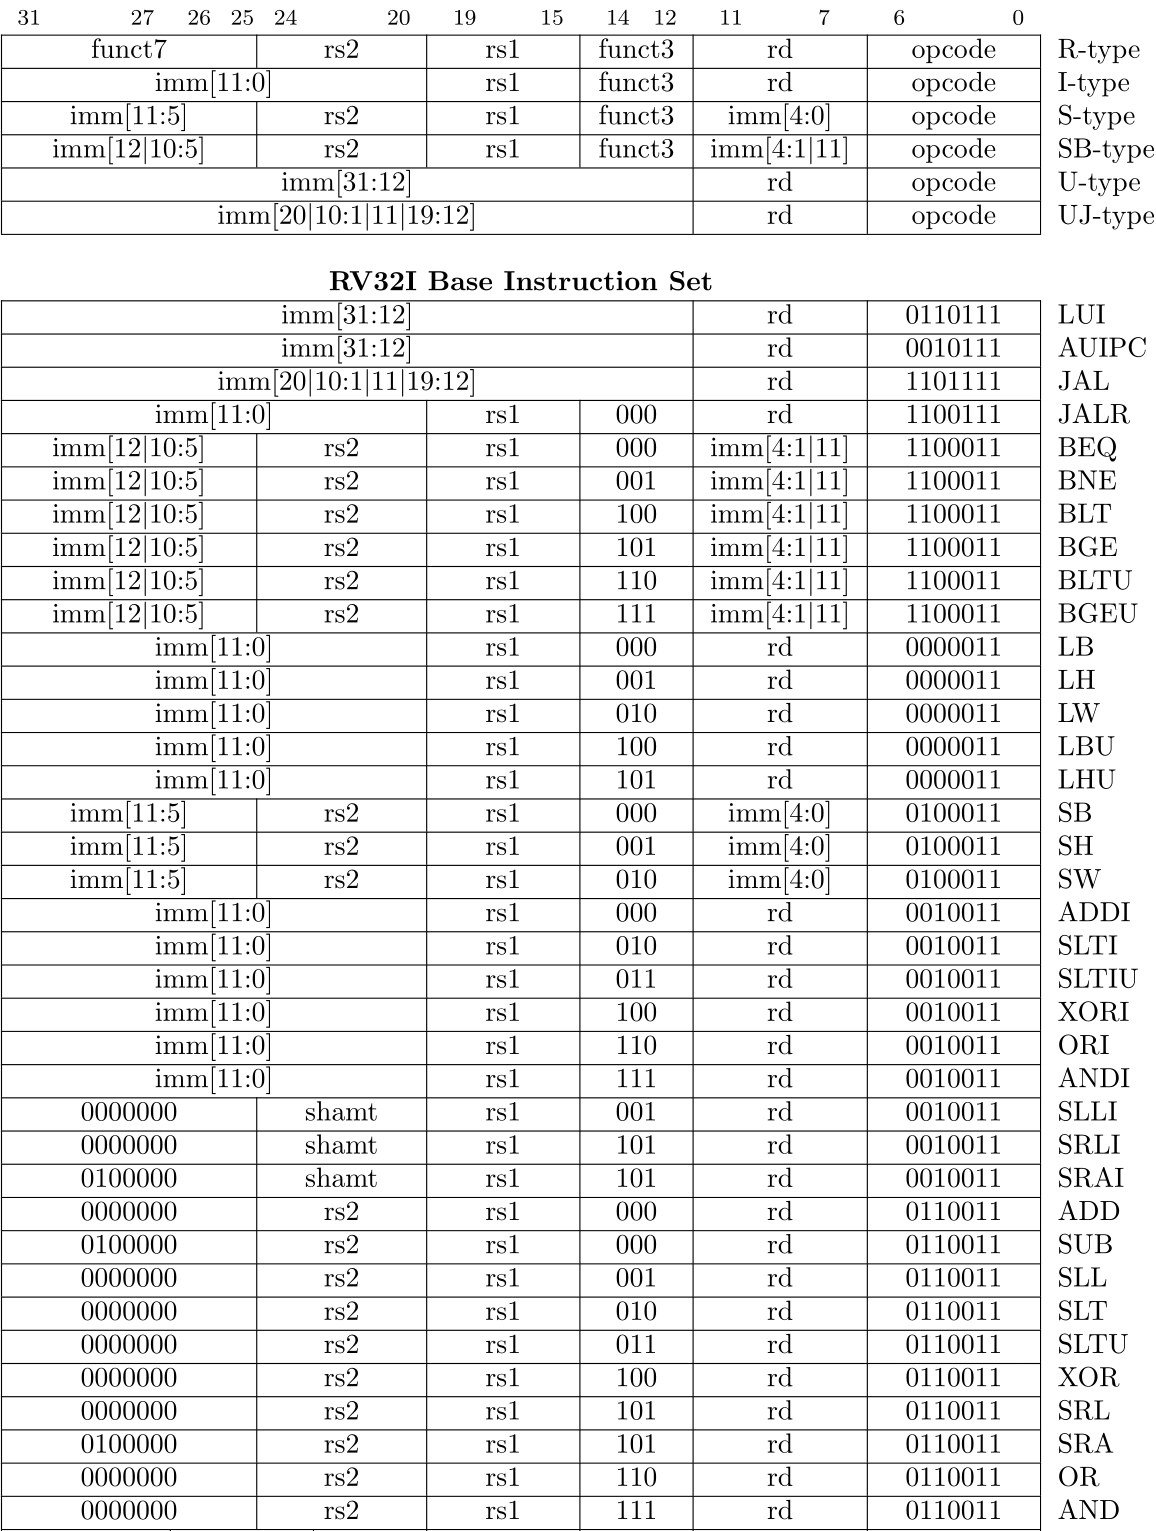
\includegraphics[width=1\textwidth]{RV32I_instr-1}
\end{center}
%\includepdf[pages=-]{RV32I_instr}

Quelle: Auszug aus der RISC-V Spezifikation \cite[S. 54]{RISC}

%----------------------------------------------------------------------------------------
%	BIBLIOGRAPHY
%----------------------------------------------------------------------------------------

\printbibliography[heading=bibintoc]

%----------------------------------------------------------------------------------------

\end{document}  
